% Forteller LaTeX at dokumentet er av typen artikkel.
% Setter også skriftstørrelsen til 11pt og papirformatet til A4.
\documentclass[a4paper,11pt]{article}

% For å kunne skrive internasjonale tegn, som æøå.
\usepackage[utf8]{inputenc}
\usepackage[T1]{fontenc}

% Fornorskning av dokumentet. Bytter f.eks. ut "Abstract" med "Sammendrag".
\usepackage[norsk]{babel}

% Fikser fet skrift og skriftstørrelse for figurtekster, tabelltekster, etc.
\usepackage[font=small,labelfont=bf]{caption}

% Inkluderer en del ekstra matematiske symboler og kommandoer.
\usepackage{amsmath}

% Inkluderer støtte for hyperlenker med kommandoen \url.
\usepackage{hyperref}

% For å kunne hente inn bildefiler til figurer.
\usepackage{graphicx}

% Inkluderer støtte for kommandoen \FloatBarrier.
% Denne kommandoen kan være til mye hjelp når det gjelder figurplassering. 
\usepackage{placeins}

% Helt i starten av dokumentet er det vanlig å ha med tittel, forfattere og dato.
\author{Andreas Sandø Krogen}
\date{\today}
\title{En kort innføring i \LaTeX}

% Her begynner selve dokumentet.
\begin{document}
% Sørger for at tittel, forfattere og dato faktisk blir skrevet i dokumentet.
\maketitle

% Sammendrag.
\begin{abstract}
Dette er en kort innføring i \LaTeX{} med hovedfokus på anvendelser i labrapportskriving. Vær oppmerksom på at denne innføringen ikke nødvendigvis er representativ for stilen akkurat din labrapport skal skrives i. Slike krav må tas opp med labveileder.
\end{abstract}

% Legger til en ny seksjon.
\section{Tekst}
Hello, World!
Legg merke til at både ekstra mellomrom    mellom ord og enkelt linjeskift ignoreres.
For å tvinge fram linjeskift kan man bruke dobbel backslash \texttt{\textbackslash\textbackslash}. \\
For nytt avsnitt, bruk to linjeskift.

Det nye avsnittet markeres normalt med innrykk. Dette kan man (hvis ønskelig) overstyre med kommandoen \texttt{\textbackslash noindent}.\\

\noindent Dette avsnittet har ikke innrykk. Som demonstrert tar \LaTeX{} seg en del friheter når det gjelder å bryte opp tekst, men noen ganger ønsker vi å overstyre dette. Et eksempel kan være at vi ikke ønsker at et linjeskift skal dukke opp i midten av et stykke tekst som bør stå sammenhengende, slik som ved forkortelser av navn. Da kan vi bruke \texttt{\textasciitilde} i stedet for mellomrom: P.~A.~M.~Dirac.

For å fullføre gjeldende side og begynne på en ny, bruk \texttt{\textbackslash newpage}.


% Legger til en ny underseksjon. Denne faller automatisk inn under forrige \section{}.
\subsection*{Tekstmarkeringer}
For \emph{uthevet} skrift, bruk \texttt{\textbackslash emph}.\\
For \textbf{fet} skrift, bruk \texttt{\textbackslash textbf}.\\
For \textit{kursiv} skrift, bruk \texttt{\textbackslash textit}.

Ofte formateres uthevet skrift og kursiv skrift likt, men noen ganger kan det hende man ønsker annen oppførsel for uthevet skrift (f.eks. annet fargevalg) og det er noe av grunnen til at vi skiller mellom disse to.

\section{Matematikk}
\LaTeX{} har ulike regler internt for hvordan ting skal se ut avhengig av om det er vanlig tekst eller matematikk. For å skrive formler i løpende tekst omslutter man formelen med \$-tegn på begge sider, som er en måte å gå inn i såkalt mattemodus (\emph{math mode}) på. Eksempler: $E = mc^2$, $v = \frac{\mathrm{d}x}{\mathrm{d}t}$.\\
% For å skrive en brøk bruker vi \frac{teller}{nevner}.
% Legg også merke til bruken av \mathrm for å få rettstilt bokstaven d.
% Når vi skriver matematikk skal variabler stå i kursiv, men resten skal som regel være rettstilt, slik som differensialtegnet i dette eksempelet.
% I mattemodus kommer bokstavene automatisk i kursiv, så det er derfor vi ved unntak må bruke \mathrm.
Hevet og senket skrift får man i mattemodus ved bruk av henholdsvis \texttt{\^\,\{hevet\}} og \texttt{\_\,\{senket\}}. For en større oversikt over matematiske symboler, sjekk ut f.eks. \url{https://en.wikibooks.org/wiki/LaTeX/Mathematics}.

\subsection{Ligninger}
For å få ligninger på egen linje med automatisk nummerering bruker vi\\ \emph{equations}-miljøet.
Man ønsker ofte å kunne henvise til ligninger, så da navngir vi dem med \texttt{\textbackslash label\{navn\}} (dette fungerer også for figurer og tabeller).\\

\begin{equation}
(x + y)^n = \sum_{k = 0}^n \binom{n}{k} x^{n-k} y^k
\label{eq:binomial}
\end{equation}

Denne kan vi nå henvise til ved hjelp av \texttt{\textbackslash eqref\{navn\}}. Vi kan også skrive ligning~\eqref{eq:binomial} uten nummerering slik

% For ligninger uten nummerering bruker vi equation* i stedet for equation.
% Tilsvarende kan vi gjøre for section, subsection, etc. ved å legge til en * på slutten.
\begin{equation*}
(x + y)^n = \sum_{k = 0}^n \binom{n}{k} x^{n-k} y^k.
\end{equation*}

Man kan skrive ligninger over flere linjer eller ha flere ligninger ordnet under hverandre, som under en utledning av noe. For dette bruker vi \emph{align}-miljøet.
% & angir hvilke tegn hver linje skal ordnes etter, slik at de ligger på samme vertikal.
% Husk \\ for linjeskift!
\begin{aligned}
x(t) &= x(0) + \int_0^t v_0 \, \mathrm{d}t^\prime \\
     &= x(0) + v_0 t \text{kg}
\end{aligned}

\section{Figurer}
\subsection{Vektorgrafikk}
Figurer som skal inkluderes i et \LaTeX{}-dokument bør være lagret som vektorgrafikk. Dette er for å hindre at bildet blir kornete under skalering. Et anbefalt gratis tegneprogram for vektorgrafikk er \texttt{Inkscape}. Eksempelfiguren under er tegnet i \texttt{Inkscape}.

\subsection{Miljøer og hvordan vi inkluderer en figur}
For å inkludere en figur bruker vi \texttt{\textbackslash includegraphics} som vi putter i et \emph{figure}-miljø. Så langt har vi brukt kommandoene \texttt{\textbackslash begin} og \texttt{\textbackslash end} ved flere anledninger, så det er på tide å redegjøre for hva de faktisk gjør. De putter ting inn i et miljø, hvor den bestemte typen miljø er gitt som argument mellom krøllparentesene. Et miljø i \LaTeX{} er (litt forenklet) en måte å si at flere ting hører sammen og derfor skal behandles som en samlet enhet. F.eks. figurer og figurtekst. Slik forhindrer vi at figuren og figurteksten havner på forskjellige sider.

Vi henviser til figurer ved hjelp av \texttt{\textbackslash ref\{figurnavn\}}.
Se figur~\ref{fig:oppsett} for et eksempel fra en tidligere labrapport i faste stoffers fysikk.
% Begynn miljø av typen figure.
\begin{figure}[htb]
% Gjør at figuren blir midtstilt.
\begin{center}
% Her angir vi bredden til figuren relativt tekstbredden i dokumentet.
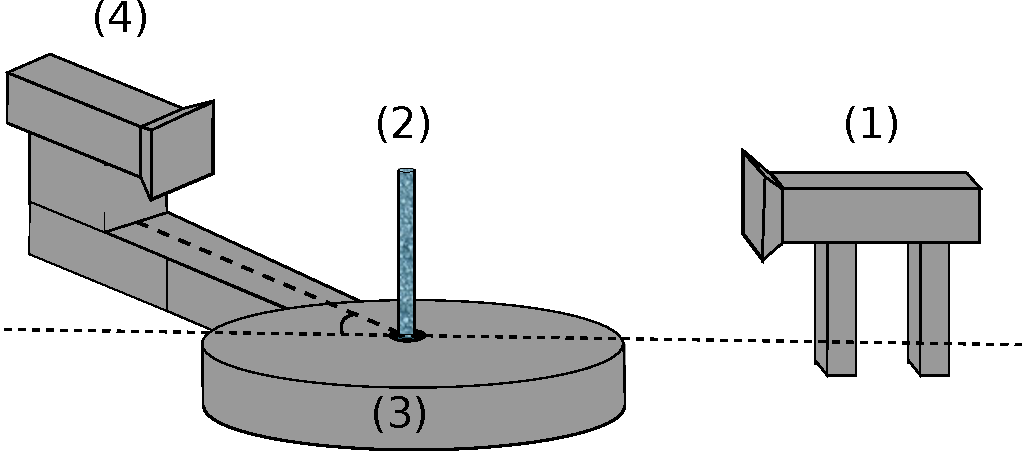
\includegraphics[width=0.8\textwidth]{oppsett.pdf}
\caption{Skisse av oppsettet. En røntgenkilde~(1) sender stråling mot en prøve~(2) som sprer strålingen mot en detektor~(4). Detektoren er festet på et goniometer~(3) som kan rotere prøven og samtidig måle vinkelutslaget.}
% Viktig at \label ligger innenfor samme miljø som selve figuren.
\label{fig:oppsett}
\end{center}
\end{figure}

% Angir at figuren ikke skal havne bak dette punktet i teksten.
\FloatBarrier

\subsection{Plassering av figurer}
Det er opp til \LaTeX{} å plassere figurene, så det er ingen garanti for at figurene havner nøyaktig der vi har definert dem i teksten. Dette kan noen ganger være en skikkelig \emph{pain in the arse}, som man sier på godt norsk. Det finnes dog noen triks. Man oppgir en prioritert rekkefølge over ønskede plasseringer slik: \texttt{\textbackslash begin\{figure\}[htb]}. Bokstaven \texttt{h} står for \emph{here} og hinter til at figuren skal plasseres omtrent der hvor den dukker opp i teksten. Bokstaven \texttt{t} står for \emph{top} og \texttt{b} står for \emph{bottom}, som hinter til at figuren skal plasseres på henholdsvis toppen og bunnen av siden.
Noe annet man kan gjøre er å legge til et utropstegn på slutten av plasseringsparametrene, f.eks. \texttt{\textbackslash begin\{figure\}[h!]}. Dette gjør at \LaTeX{} ignorer enkelte av sine interne regler for hvordan figurene ``best'' skal plasseres, slik at de (forhåpentligvis) dukker opp der man ønsker i teksten.
Noen ganger fungerer ikke engang dette slik man ønsker, men det finnes enda et triks: I pakken \texttt{placeins} er det en kommando som heter \texttt{\textbackslash FloatBarrier} (pass på små og store bokstaver!). Denne tvinger alle hittil definerte flytende miljøer, som figurer og tabeller, til å bli plassert før \texttt{\textbackslash FloatBarrier} i teksten.

Et godt tips er å ikke bruke for mye tid på å styre med figurplasseringer før man har fått på plass resten av innholdet. Å legge til nytt innhold kan fort ha innvirkning på hvor figurene havner, og da er man tilbake der man startet.

Vær også oppmerksom på at ikke alle bildefilformater støttes. Vektorgrafikk fra Inkscape eksporteres som regel til PDF-format, noe som skal fungere, og det skal være mulig å inkludere bilder i formatene PNG og JPG.


\section{Tabeller}
Tabeller opprettes med \emph{tabular}-miljøet, som igjen gjerne plasseres inne i et \emph{table}-miljø for å få automatisk nummerering og tabelltekst. Plassering og henvisninger fungerer på lik måte for tabeller som for figurer. Viser til tabell~\ref{tab:SI-enheter} som eksempel. Ved opprettelsen av et \emph{tabular}-miljø må man spesifisere antall kolonner, samt hvordan elementene i tabellen skal være justert. Eksempel: \texttt{\textbackslash begin\{tabular\}\{l c r\}}. Her har vi tre bokstaver; én for hver kolonne. Bokstaven \texttt{l} angir at første kolonne skal være venstrejustert, \texttt{c} at andre kolonne skal være midtstilt og \texttt{r} at tredje kolonne skal være høyrejustert.

\begin{table}[h!]
% Midtstiller tabellen.
\centering
% Tabellteksten skal komme før tabellen.
\caption{SI-enheter}

\begin{tabular}{l c l}
% Her legger vi til litt tomrom mellom den første horisontale linjen \hline og første rad
% i tabellen, slik at det skal se penere ut.
% Dette fungerer ved at vi bruker \\ for linjeskift, men med parameteren -4mm som
% krymper et fullt linjeskift med 4mm, da det ellers ville blitt litt for mye tomrom.
\hline \\[-4mm]
% Elementene i hver rad skilles av et &-tegn.
\emph{Størrelse} & \emph{Navn} & \emph{Symbol} \\
\hline
lengde      & meter    & m \\
masse       & kilogram & kg \\
tid         & sekund   & s \\
strøm       & ampere   & A \\
temperatur  & kelvin   & K \\
stoffmengde & mol      & mol \\
lysstyrke   & candela  & Cd \\ \hline
\end{tabular}
% En annen måte å legge til vertikalt tomrom i f.eks. tabeller er med \vspace.
% Eksempel: \vspace{4mm}.
% For fullstendighetens skyld: Det finnes en tilsvarende kommando for horisontalt tomrom,
% kalt \hspace.
\label{tab:SI-enheter}
\end{table}

Legg merke til at enheter skal skrives med rettstilt skrift.

\section{Kildehenvisninger og fotnoter}
I enhver vitenskapelig tekst er det viktig å oppgi hvilke kilder man har benyttet seg av på en måte som gjør at leseren lett kan finne fram til dem og ettergå at de faktisk holder vann. Derfor inkluderer vi en kildeliste i slutten av dokumentet. For å opprette en kildeliste med kilder som vi kan henvise til i teksten bruker vi \emph{thebibliography}-miljøet. Innenfor miljøet kan vi legge til kilder med \texttt{\textbackslash bibitem\{kildenavn\}} etterfulgt av selve kilden. For å henvise til kilden bruker vi \texttt{\textbackslash cite\{kildenavn\}}.\\
Eksempel: Videre kvantiseres systemet som foreslått av Dirac~\cite{dirac}.

Noen ganger kan det hende vi ønsker å komme med en liten sidekommentar, samtidig som vi ikke ønsker å ødelegge tekstflyten. Da kan vi benytte oss av fotnoter som opprettes med kommandoen \texttt{\textbackslash footnote\{tekst\}}.\footnote{Dette er en fotnote.}

Til slutt en liten kommentar som kanskje kan spare noen for litt forvirring:
Når man har et \LaTeX{}-dokument med henvisninger, så må man noen ganger kompilere dokumentet to ganger etter hverandre for at henvisningene skal bli plassert inn korrekt. Etter første kompilering kan det altså hende at det i stedet for de riktige figurtallene, ligningstallene, etc. kun står to spørsmålstegn.

% Bibliografi. Her fører vi opp kilder som vi kan henvise til ellers i dokumentet.
\begin{thebibliography}{10}
\bibitem{dirac} P.~A.~M.~Dirac, \textsc{the quantum theory of the emission and absorption of radiation}, \textit{Proceedings of the Royal Society of London}, Series A, Vol. 114, p. 243 (1927)
\end{thebibliography}

\newpage
\section*{Takksigelser}
Takk til Birk Engegård for snasen eksempelfigur og til Jon Andreas Støvneng som tidligere har gitt en introduksjon til \LaTeX{} som jeg har hentet inspirasjon fra.~\footnote{\url{http://web.phys.ntnu.no/~stovneng/TFY4145_2015/oppstart/latex.htm}}
\end{document}\grid
